\section{Implementation and Evaluation}

We implemented drone-side speech processing on a small embedded audio platform. The setup uses a XIAO ESP32-S3 Sense board placed near the drone, with the board microphone capturing nearby speech. Each input is a one-second window of 16~kHz mono audio. The speech processor first converts the waveform into log-mel time-frequency features. A compact neural classifier, with a small convolutional frontend followed by temporal sequence modeling, then processes these features onboard and returns a safety-net category: \emph{emergency}, \emph{movement}, or \emph{unknown}.

The controlled recognition experiments use Google Speech Commands utterances mapped into the three safety-net categories and mixed with locally captured drone rotor audio. The participant study is used only for live onboard evaluation, not for training.

\begin{figure*}[t]
    \centering
    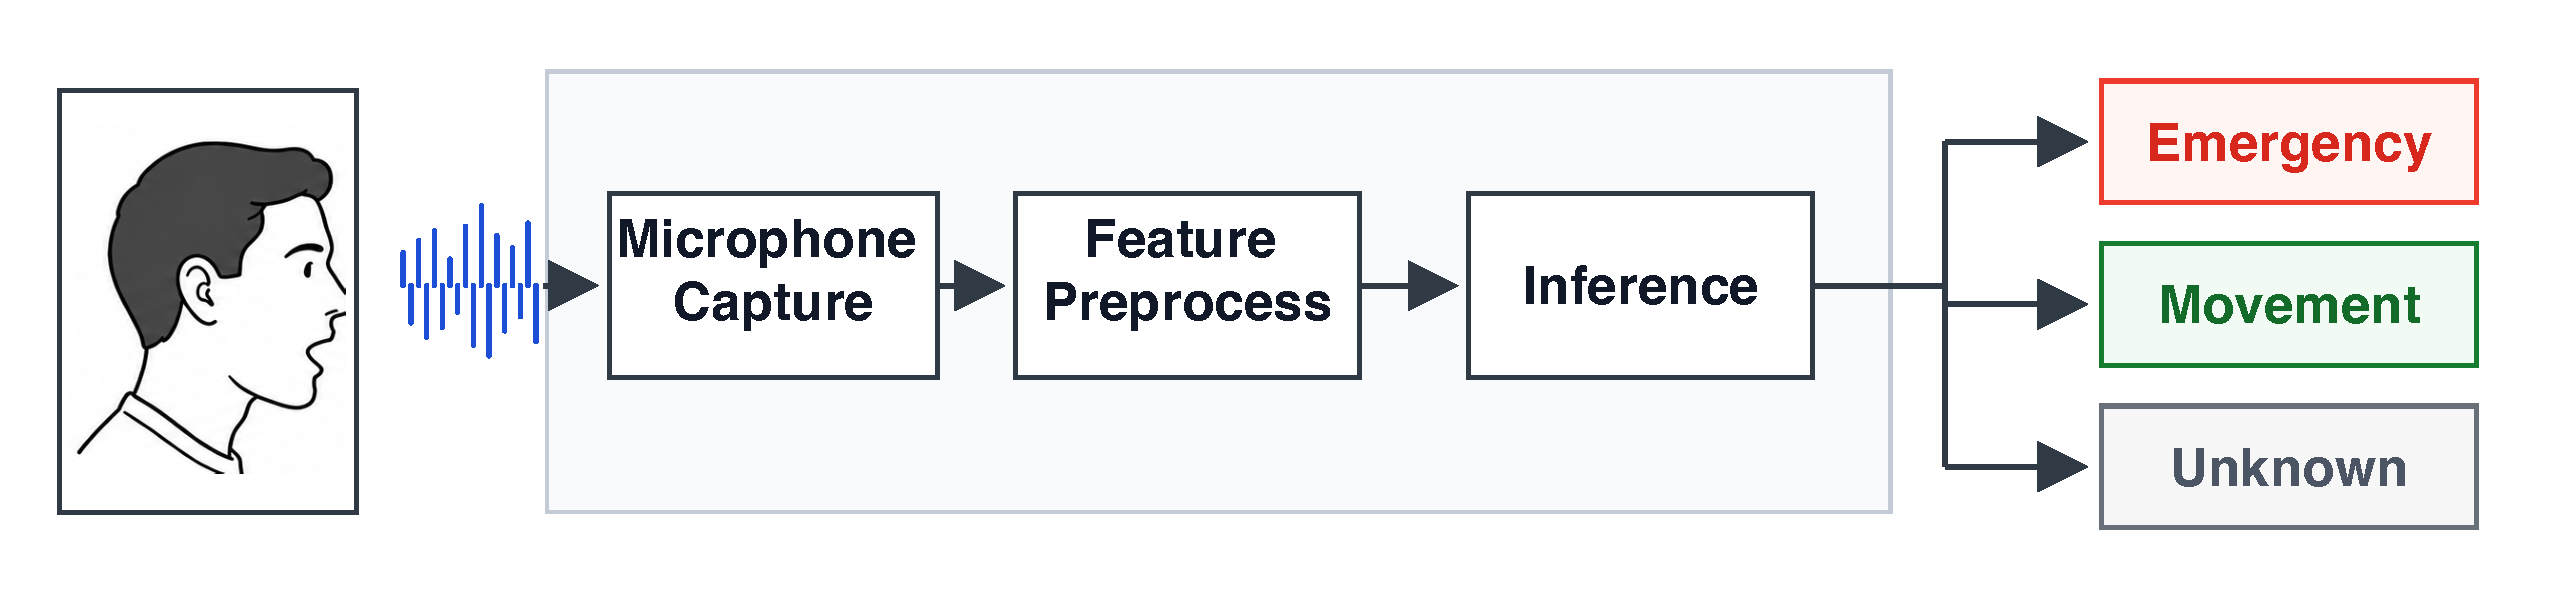
\includegraphics[width=\textwidth]{figures/onboard_speech_pipeline.pdf}
    \caption{Drone-side speech-processing pipeline.}
    \label{fig:onboard_speech_pipeline}
\end{figure*}

Figure~\ref{fig:onboard_speech_pipeline} shows the drone-side pipeline. Nearby speech is captured by the microphone on the XIAO ESP32-S3 Sense board, keeping sensing close to the drone's acoustic condition, including rotor noise, microphone placement, and the changing geometry between the speaker and vehicle. The captured audio is then converted into log-mel features and passed to the onboard classifier for real-time inference. The pipeline ends with one of three safety-net categories: \emph{emergency}, \emph{movement}, or \emph{unknown}. Because this first interpretation runs locally, the interaction does not depend on a phone application, cloud speech service, or reliable network path at the moment when nearby speech is produced.

This implementation is intentionally narrow. It does not attempt to parse open-ended language, estimate a complete dialogue state, or decide how the drone should move. It focuses on the first part of the safety-net path: can the drone-side device listen in the relevant acoustic setting and produce a compact speech-derived signal quickly enough to be useful? 

We summarize four kinds of evaluation evidence. First, we test the speech module under different rotor-noise SNR conditions to show how changes in the acoustic environment affect speech processing. Second, we compare the safety-net speech-processing design with conventional alternatives, including transcript-first and compact command-recognition baselines, to explain why speech-derived safety-net categories are a more suitable first handoff for spoken drone interaction. Third, we report the embedded runtime behavior to show whether the XIAO ESP32-S3 Sense path can sustain local sensing, feature processing, and inference. Fourth, we report participant-level live speech trials to expose how the onboard path varies across speakers.

\begin{table}[t]
    \centering
    \caption{Speech-processing output under different rotor-noise SNR conditions.}
    \label{tab:snr_results}
    \footnotesize
    \setlength{\tabcolsep}{3pt}
    \begin{tabular}{@{}lcc@{}}
        \toprule
        SNR & Acc. & Emerg. recall \\
        \midrule
        -10~dB & 0.86 & 0.86 \\
        -15~dB & 0.83 & 0.85 \\
        -20~dB & 0.76 & 0.81 \\
        \bottomrule
    \end{tabular}
\end{table}

Table~\ref{tab:snr_results} shows how the speech module changes as rotor noise becomes stronger. Accuracy decreases as the SNR moves from -10~dB to -20~dB, while emergency recall remains at or above 0.81 across the tested conditions. This trend is important for the article's framing: spoken drone interaction is shaped by the acoustic environment, so the safety net should begin with a speech-derived category that is explicit about what the audio system can and cannot separate under noise.

\begin{table}[t]
    \centering
    \caption{Comparison with transcript-first and compact command-recognition baselines on rotor-noisy one-second clips at -10~dB SNR.}
    \label{tab:baseline_comparison}
    \footnotesize
    \setlength{\tabcolsep}{3pt}
    \begin{tabular}{@{}p{0.48\linewidth}cc@{}}
        \toprule
        Method & Acc. & Emerg. recall \\
        \midrule
        Drone-side speech processor & 0.86 & 0.86 \\
        Whisper \texttt{tiny.en} + parser & 0.43 & 0.22 \\
        DS-CNN-S family & 0.61 & 0.78 \\
        \bottomrule
    \end{tabular}
\end{table}

Table~\ref{tab:baseline_comparison} explains why the system is framed around speech processing for a safety net rather than raw transcripts or ordinary command recognition at the -10~dB comparison point. The transcript-first pipeline performs poorly on the short noisy windows because it must first recover usable text before the safety-net category can be inferred. The compact command-recognition baseline is closer to the proposed path, but it still treats the audio problem as ordinary label selection. The drone-side speech processor instead makes the output match the interaction need: separating emergency speech, movement-related speech, and unsupported input before later drone-facing decisions are considered.

The embedded runtime result checks whether this pipeline can run locally. In a dual-core onboard timing run over 120 one-second windows, more than 95\% of clips were processed at approximately the one-second window rate after the first update, with no dropped or overrun windows.

We also collected live speech from 11 participants using the same onboard capture-to-inference path. The study included prompted utterances across the three safety-net categories and produced 1462 total samples. Table~\ref{tab:participant_live_trials} reports participant-level emergency recall and overall accuracy. The lower emergency recall in these live trials should be read together with the controlled SNR results. The SNR tests use fixed one-second clips under controlled mixtures, while the participant trials introduce live speech variation, including speaking rate, pronunciation, delivery, microphone alignment, and collection-condition mismatch. The relatively large standard deviation therefore highlights cross-speaker variability, which motivates the cross-user robustness work discussed in Section~V.


\begin{figure*}[t]
    \centering
    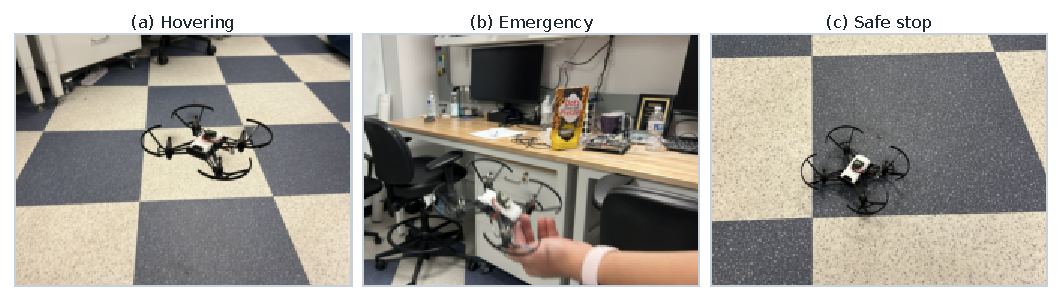
\includegraphics[width=\textwidth]{figures/emergency_stop_sequence.pdf}
    \caption{Emergency-related speech demonstration scene. A nearby person speaks toward the drone, the onboard pipeline continues processing local audio, and the system presents the detected emergency-related speech as the relevant safety-net signal for the scene.}
    \label{fig:emergency_demo}
\end{figure*}

Figure~\ref{fig:emergency_demo} shows the setting behind the emergency case. A person near the drone produces urgent speech, the drone-side audio pipeline processes the input locally, and the output is treated as emergency-related speech rather than as an open-ended transcript or ordinary movement command. This scene shows how the safety-net framing appears in a concrete spoken-drone interaction.

\begin{table}[t]
    \centering
    \caption{Participant-level user study using onboard capture and inference.}
    \label{tab:participant_live_trials}
    \footnotesize
    \setlength{\tabcolsep}{4pt}
    \begin{tabular}{@{}lccc@{}}
        \toprule
        Speakers & Number of Samples & Emerg. recall & Acc. \\
        \midrule
        11 & 1462 & 0.623 $\pm$ 0.148 & 0.764 $\pm$ 0.079 \\
        \bottomrule
    \end{tabular}
\end{table}
